\documentclass[]{article}
\usepackage{graphicx}
\usepackage{float}

%opening
\title{Asteroids: a 2d game that let you shoot asteroids and other objects while piloting your spaceship in the space }
\author{Kareem Salah, Belal Ibrahim, Khaled Hesham, Mostafa Hazem}

\begin{document}

\maketitle
\noindent\rule{12cm}{0.5pt}

\section{PROJECT FUNCTIONALITIES}

\subsection{Initialize}
Initialize the states of the game

\subsection{Render}
Responsible for rendering the changes happen in the game

\subsection{Fire}
Make the player able to shoot projectile with appropriate physics

\subsection{Projectile Collision}
Handle whenever projectile hit an object

\subsection{Player Collision}
Handle whenever the player collides with obstacle

\subsection{Move Obstacle}
Move obstacles with the appropriate inertia

\subsection{Move Player}
Move Player with the appropriate inertia

\subsection{Move Projectile}
Move Projectile with the appropriate inertia

\subsection{Thrust}
key-event that control speed for player space-ship

\subsection{Change Direction}
key-event that let you change the direction where your spaceship is looking

\subsection{Add Obstacle}
add new obstacles to make game harder overtime 

\noindent\rule{12cm}{0.5pt}

\begin{itemize}

  \item Kareem Salah, 20150388,
  \newline
  E-mail: karim.salah2048@gmail.com
  
  \item Belal Ibrahim, 20150186,
  \newline
  E-mail: billyfcih@yahoo.com
  
  \item Khaled Hesham, 20150226
  \newline
  E-mail: khaledhesham2017@hotmail.com
  
  \item Mostafa Hazem, 20150528
  \newline
  E-mail: mostafahazem144@yahoo.com
  
\end{itemize}
Programming Language 3 - CS313 - Spring 2017 - Faculty of
Computers and Information - Helwan University

\section{Project Backlog}

\subsection{DEVELOPMENT}

\begin{figure}[H]
\centering
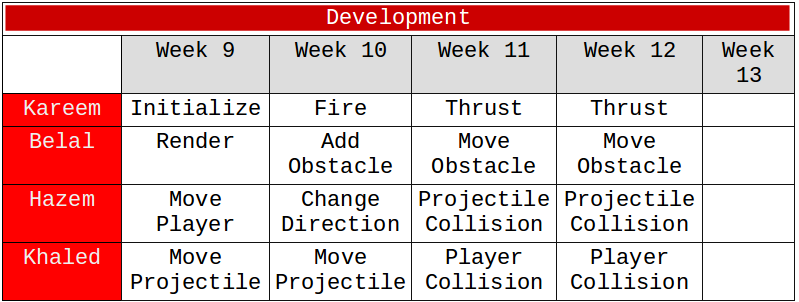
\includegraphics[scale=0.5]{./Develop.png}
\end{figure}

\subsection{TESTING}

\begin{figure}[H]
\centering
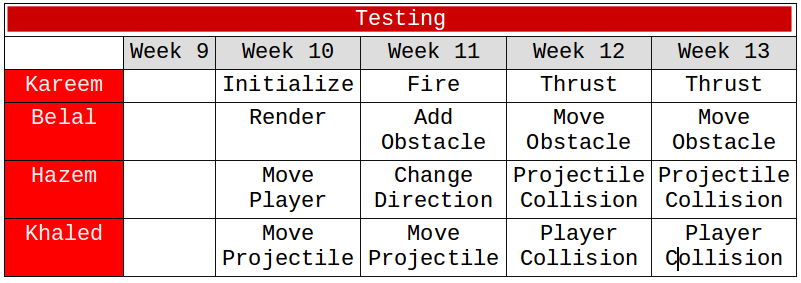
\includegraphics[scale=0.5]{./Test.png}
\end{figure}

\end{document}